\documentclass[10pt, hyperref={unicode}, xcolor=dvipsnames]{beamer}
\usepackage[slovak]{babel}
\usepackage[utf8]{inputenc}
\usepackage{times} 
\usepackage{graphics} 
\usepackage{hyperref}
\usepackage{url}
\usepackage[ruled, czech, noline, linesnumbered, noend]{algorithm2e}
\usepackage{listings}

\useoutertheme{shadow}
\setbeamertemplate{headline}{}

\usetheme{Copenhagen}
\usecolortheme{seahorse}

\title{Dijkstrov algoritmus}
\subtitle{Typografie a~publikování 5. projekt}
\author{Simona Jánošíková}
\date{\today}
\institute{
    Vysoké učení technické v~Brně\\
    Fakulta informačních technologií
}

\begin{document}
\frame{
    \maketitle
}

\frame{
    \frametitle{Obsah}
    \tableofcontents
}

\frame{
    \frametitle{Dijkstrov algoritmus}
    \section{Dijkstrov algoritmus}
    \begin{itemize}
        \item Slúži k vyhľadaniu najkratšej cesty v~grafe medzi dvoma vrcholmi.
        \item Autorom tohto algoritmu je holandský matematik E. W. Dijkstra.
        \item Je konečný, čiže algoritmus vždy skončí pre ľubovolný konečný vstup.
        \item Pre správnu funkcionalitu algoritmus očakáva orientovaný, ohodnotený graf so všetkými hranami ohodnotenými kladne.
    \end{itemize}
}

\frame{
    \frametitle{Princíp}
    \section{Princíp}
    \begin{itemize}
        \item Majme graf \textbf{G}, množinu všetkých vrcholov \textbf{V}, množinu všetkých hrán \textbf{E}, množinu navštívaných vrcholov \textbf{Z} a množinu ešte nenavštívaných vrcholov \textbf{N}.
        \item Pre každý vrchol \textbf{v} z \textbf{V} si algoritmus pamätá dĺžku najkratšej cesty, označujeme $\textbf{d[v]}$, ako sa k nemu dostať.
        \item V každom cykle sa pridá jeden vrchol z \textbf{N}, $v_{min}$ s najmenšou hodnotou $\textbf{d[v]}$, do \textbf{Z}.
        \item Algoritmus pracuje v cyklu tak dlho, pokiaľ \textbf{N} nie je prázdna. 
        \item Po skončení algorytmu je pre každý vrchol \textbf{v} uložená dĺžka najkratšej cesty od počiatočného vrcholu \textbf{s} v $\textbf{d[v]}$.
    \end{itemize}
}

\frame{
    \begin{figure}[h]
        \begin{center}
            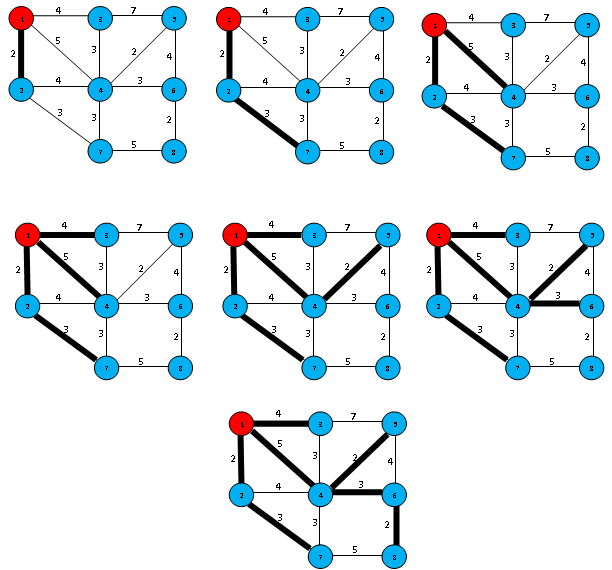
\includegraphics[width=1\textwidth,height=0.8\textheight,keepaspectratio]{algorithm.png}
        \end{center}
    \end{figure}
}

\frame{
    \frametitle{Pseudokód}
    \section{Pseudokód}
    \IncMargin{1.5em}
    \begin{algorithm}[H]
        \caption{\textsc{Dijkstra}}
		\SetKwFunction{FMain}{Dijkstra}
		\SetKwProg{Pn}{function}{:}{\KwRet}
        \Pn{\FMain{E, V, s}}{
            \ForEach{vertex v \textbf{in} V}{
                d[v] := infinity\\
                p[v] := undefined\\
            }
            d[s] := 0\\
            N := V\\
            \While{N \textbf{is not} empty}{
                u := extract\textunderscore min(N)\\                
                \ForEach{neighbor v \textbf{of} u}{
                    alt = d[u] + l(u, v)\\
                    \uIf{alt \textless \,d[v]}{
                        d[v] := alt\\
                        p[v] := u\\
                    }
                }
            }
        }
    \end{algorithm}
}

\section{Časová zložitosť}
\frame{
    \frametitle{Časová zložitosť}
    \begin{itemize}
        \item Ak je dijsktrov algoritmus implementovaný pomocou prioritnej fronty, tak jeho časová zložitosť je asymtotická $O(n^2)$, kde $n$ značí počet operácií.
        \pause
        \item Pre riedke grafy je efektívnejšia implementácia pomocou binárnej haldy s časovou zložitosťou $O((n+m)\log (n))$ alebo s použitím Fibonacciho haldy je časová zložitosť $O(n\log (n) + m)$, kde $n$ je počet vrcholov a $m$ je počet hrán grafu.
    \end{itemize}
}

\frame{
    \frametitle{Použité zdroje}
    \section*{Použité zdroje}
    \begin{itemize}
        \item Wikipedia.org - Dijktrův algoritmus\\
        \href{https://cs.wikipedia.org/wiki/Dijkstrův_algoritmus}{\small{\texttt{https://cs.wikipedia.org/wiki/Dijkstrův\textunderscore algoritmus}}}
    \end{itemize}
}


\end{document}
